\section{Generativní modelování obrazových dat}
\label{sec:applications_generative_modeling}
Generativní modelování přirozených obrázků představuje jednu z nejaktuálnějších úloh učení bez učitele vůbec.
VAE (a jeho rozšíření) natrénované na datasetech obrazových dat v této oblasti dosahují excelentních výsledků \cite{Gulrajani2016}.
DRAW (rozšíření VAE, viz \autoref{sec:draw}) je jedna z vůbec prvních architektur VAE modifikovaná k generování \textbf{zcela nových a realistických obrázků}, jenž nebyly součástí trénovací množiny.
Vygenerované výstupy zachycuje \autoref{fig:mnist_double_digits_gregor}.

\begin{figure}[H]
    \centering
    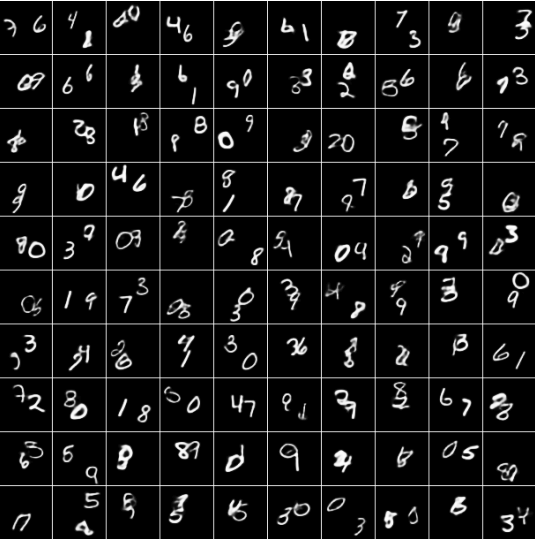
\includegraphics[width=0.55\textwidth]{figures/applications/mnist_double_digits_gregor.png}
    \caption{Aplikace VAE na generování zcela nových obrázků dvou cifer, trénováno na MNIST datasetu. Převzato z \textcite{Gregor2015}.}
    \label{fig:mnist_double_digits_gregor}
\end{figure}

Další rozšířenou architekturou je PixelVAE \cite{Gulrajani2016}, která oproti DRAW nabízí větší kvalitu realistických obrázků vzorkovaných z generativního modelu.
Její výstupy prezentuje \autoref{fig:image_net_pixel_vae_gulrajani}.

\begin{figure}[H]
    \centering
    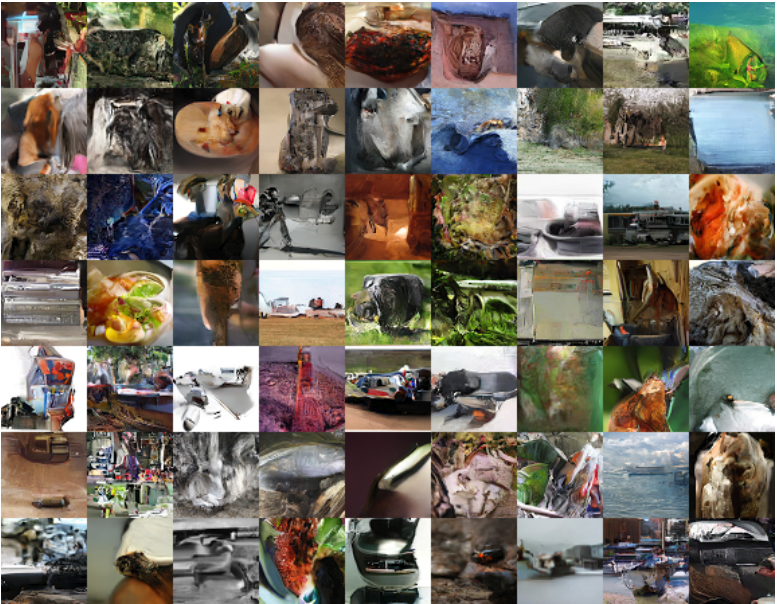
\includegraphics[width=0.55\textwidth]{figures/applications/image_net_pixel_vae_gulrajani.png}
    \caption{Výsledek vzorkování PixelVAE \cite{Gulrajani2016}, ImageNet dataset.}
    \label{fig:image_net_pixel_vae_gulrajani}
\end{figure}

\newpage
\section{Opakovaná syntéza obrazových dat}
\label{sec:applications_image_resynthesis}
Populární aplikací VAE je (re)syntéza obrazových dat.
Využití jednoduchého modelu VAE k opakované syntéze obrazových dat (konkrétně snímků lidských obličejů) představuje \textcite{White2016}.

VAE lze optimalizovat za účelem zformování generativního modelu skrze vstupní sadu obrazových dat.
Z takového generativního modelu pak lze vzorkovat zcela nové obrázky, které nebyly součástí trénovací množiny dat. \cite{Kingma2019}

\begin{figure}[H]
    \centering
    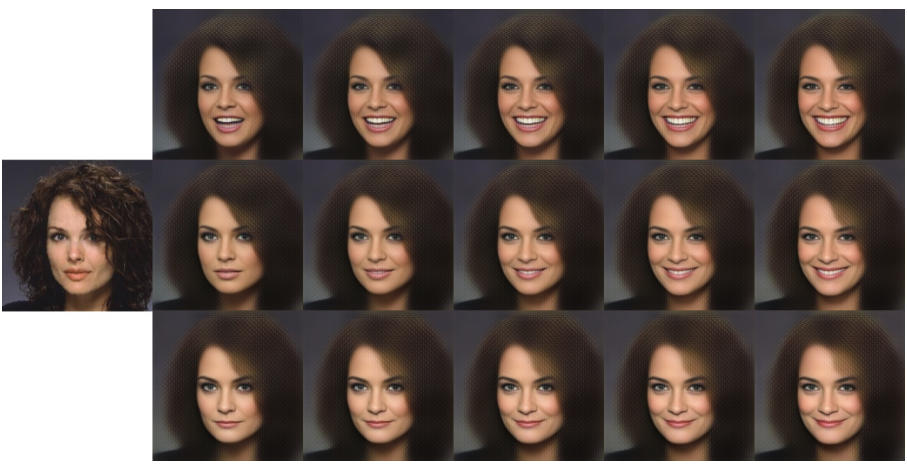
\includegraphics[width=\textwidth]{figures/applications/vae_smile_vector_white.png}
    \caption{Využití VAE pro opakovanou syntézu vstupního obrázku. V tomto příkladě lze pozorovat posun původního obrázku (vlevo) v modifikovaném latentním prostoru ve směru \emph{vektoru úsměvu} (tzv. aritmetika v latentním prostoru), což má za výsledek progresivně více usmívající se obličej. Převzato z \textcite{White2016}.}
    \label{fig:vae_smile_vector_white}
\end{figure}


\textbf{Takto naučený model ale nabízí ještě jednu zajímavou aplikaci}.
Inferenční model (enkodér) totiž umožňuje zakódovat reálné obrázky do jeho latentního prostoru.
Tento kód pak lze ve vzniklém latentní prostoru modifikovat a následně jej dekódovat zpět do pozorovaného prostoru.
Aplikace jednoduchých transformací – například pouhé lineární transformace – na tento prostor má často za důsledek \textbf{sémanticky významnou modifikaci původního obrázku}.
\autoref{fig:vae_smile_vector_white} demonstruje modifikaci obrázku obličeje v latentním prostoru podél \textbf{"vektoru úsměvu"}, což činí původní obrázek progresivně více veselejším (lze pozorovat i osu \emph{otevřených úst} při úsměvu). \cite{Kingma2019}

\newpage
\section{Kolorování obrázků}
\label{sec:applications_image_coloring}
Další slibnou aplikací VAE v oblasti generativního modelování obrazových dat je predikce původní barvy jednotlivých pixelů obrázku na základě černobílého (\emph{gray~scale}) vstupu.

V \textcite{Deshpande2017} autoři představují architekturu VAE, která rozšiřuje CVAE a modifikuje jeho ztrátovou funkci (a to za účelem zpřesnění predikce barvy pixelů a vyhnutí se rozostřeným vygenerovaným vzorkům).
\begin{figure}[H]
    \centering
    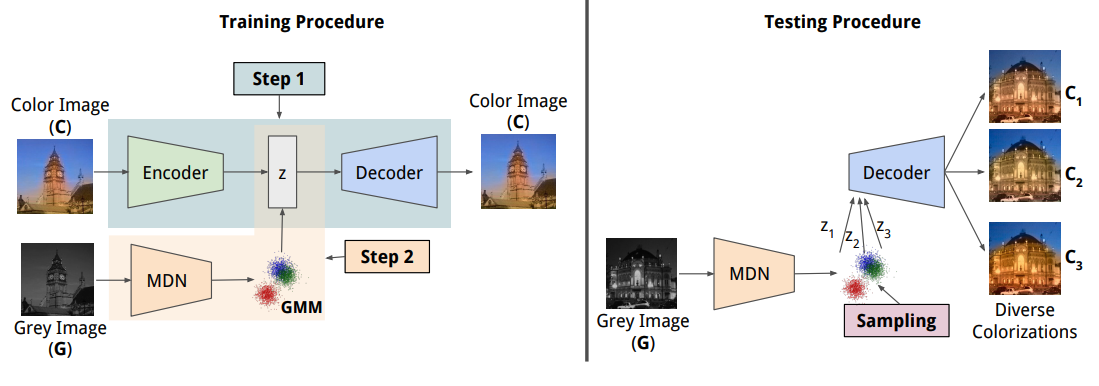
\includegraphics[width=0.9\textwidth]{figures/applications/predicting_pixel_colors_deshpande_vae_schema.png}
    \caption{Schéma trénovací a vzorkovací procedury rozšířeného CVAE pro predikci barvy pixelů původního obrázku. Převzato z \textcite{Deshpande2017}.}
    \label{fig:predicting_pixel_colors_deshpande_schema}
\end{figure}

V trénovací fázi se jako první model naučí nízkodimenzionální reprezentaci $z$ pro barevné pole $C$.
Poté je natrénován podmíněný pravděpodobnostní model $P(z \mid G)$, který generuje nízkodimenzionální reprezentaci na základě černobílého vstupu $G$. 
Tento pravděpodobnostní model lze poté vzorkovat a využít dekodér modul vzniklého VAE pro vygenerování rozmanitých barevných polí původního obrázku na výstupu (tj. vygenerování více kombinací \emph{obarvení} gray~scale obrázku).
\textbf{Při vzorkování generativní model jako vstup obdrží pouze gray~scale obrázek}. Schéma procedur tohoto modelu zachycuje \autoref{fig:predicting_pixel_colors_deshpande_schema}. \cite{Deshpande2017}

\begin{figure}[H]
    \centering
    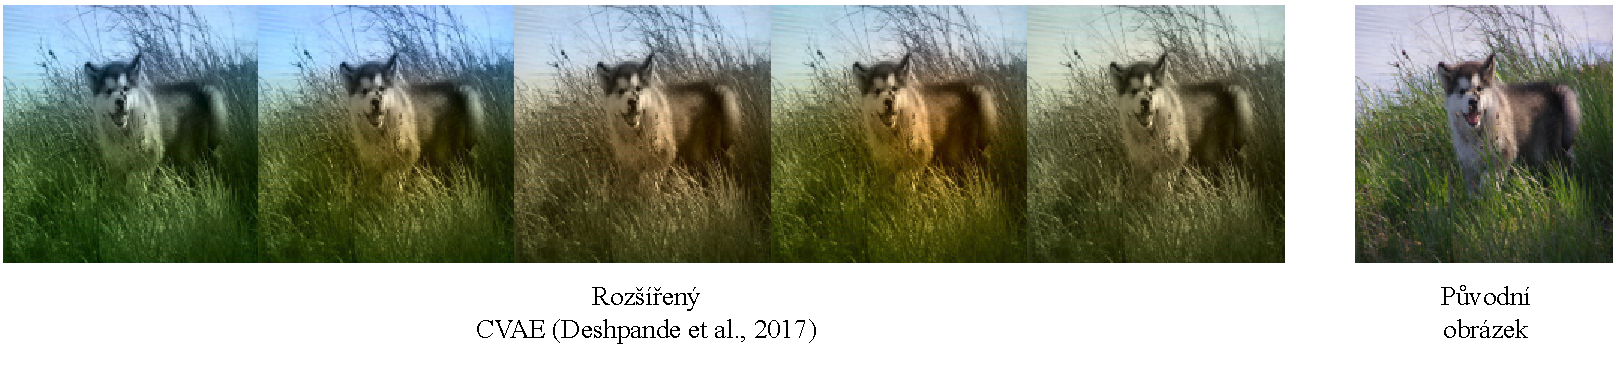
\includegraphics[width=0.9\textwidth]{figures/applications/predicting_pixel_colors_deshpande.pdf}
    \caption{Vzorek vygenerovaných variací (vlevo) obarvení původního obrázku (vpravo). Vstupem pro generativní model byl \textbf{pouze černobílý} obrázek. Převzato z \textcite{Deshpande2017}.}
    \label{fig:predicting_pixel_colors_deshpande}
\end{figure}

\autoref{fig:predicting_pixel_colors_deshpande} prezentuje vzniklé variace obarvení původního obrázku na základě černobílého vstupu.
Takto naučený model tedy lze využít například k obarvení černobílých fotografií.

\newpage
\section{Rekonstrukce obrazových dat}
\label{sec:applications_image_reconstruction}
Mechanismus VAE je možné využít rovněž k \textbf{rekonstrukci} obrazových dat – tedy doplnění chybějící části obrázku generativním modelem (tzv. \emph{inpainting}).
Autoři \textcite{Yan2016} představují aplikaci VAE (a jeho rozšíření) v kontextu generativního modelování podmíněného atributem (\emph{attribute-conditioned generative modeling}).

\begin{figure}[H]
    \centering
    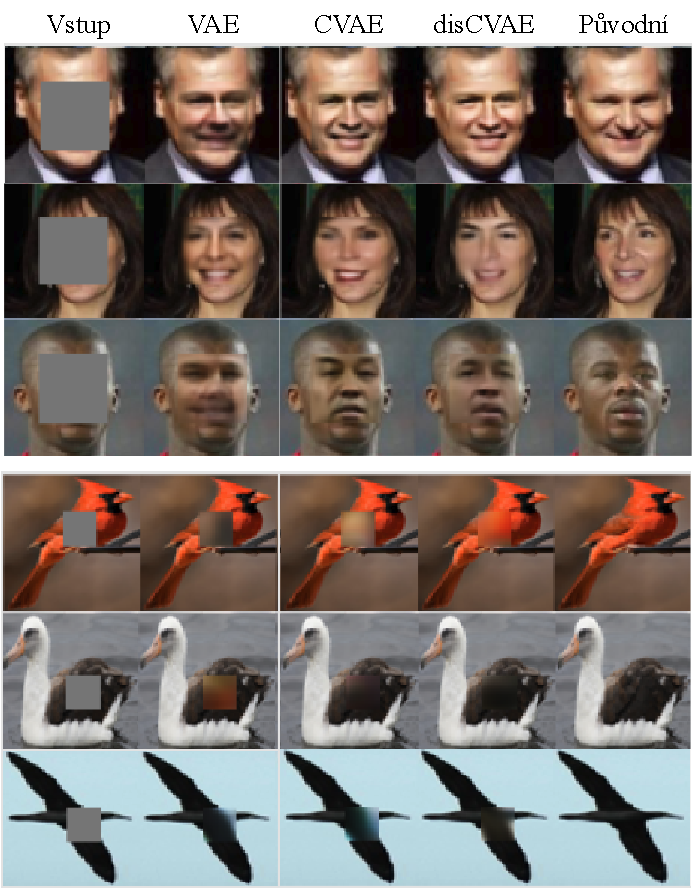
\includegraphics[width=0.65\textwidth]{figures/applications/image_inpainting_yan.pdf}
    \caption{Výstup modelů VAE pro rekonstrukci dat. Převzato z \textcite{Yan2016}.}
    \label{fig:image_inpainting_yan}
\end{figure}

Předložený model je naučen na nepoškozených datech. Jako \textbf{vstup} pro generativní proces slouží \textbf{neúplný obrázek}.
Cílem generativního modelu je předpovědět kontext chybějícího regionu obrázku a s ohledem na zbylou část správně doplnit jeho obsah. \cite{Yan2016}

\autoref{fig:image_inpainting_yan} prezentuje výstupy modelů VAE aplikovaných na rekonstrukci chybějících regionů \textbf{přirozených} obrazových dat.
Obrázek nahoře prezentuje výsledky generativního procesu podmíněného atributem obličeje (model je trénován na datasetu LFW \footnote{Labeled Faces in the Wild. \cite{Huang2012}}).
Obrázek dole pak výsledky které nejsou podmíněny žádným atributem – chybějící region obrázku ($16\times16$ px) je vybrán náhodně (model je trénován na datasetu CUB \footnote{Caltech-UCSD Birds-200-2011. \cite{Wah2011}}).

\newpage
\section{Konceptuální komprese}
Další aplikací VAE je konceptuální komprese \cite{Gregor2016}. Úloha je úzce spjata s informační teorií a interpretací VAE z pohledu informační teorie (viz \autoref{sec:vae_information_theory_interpretation}).

Chceme-li komprimovat obrázky psů a koček na jeden bit, jak by měl tento bit vypadat?
Dalo by se předpokládat, že by měl ukládat informaci, zda-li se na obrázku nachází pes, či kočka. 
Na základě této jediné latentní proměnné pak generativní model vygeneruje kompletní obrázek.
Uvažujme nyní, že místo jednoho bitu chceme provést kompresi na 10 bitů.
Lze tedy uložit ty nejvíce stěžejní vlastnosti o vyobrazeném objektu  – například barvu, natočení objektu a podobně.
Zbývající (detailnější) vlastnosti – jako například vzor srsti – opět \emph{doplní} generativní model (který na základě těchto informací podmíníme, viz \autoref{sec:cvae}).
Čím větší počet proměnných v latentním prostoru (čím více bitů má cílová komprese), tím více informací je možné o původním objektu zachovat. \cite{Gregor2016}

\begin{figure}[H]
    \centering
    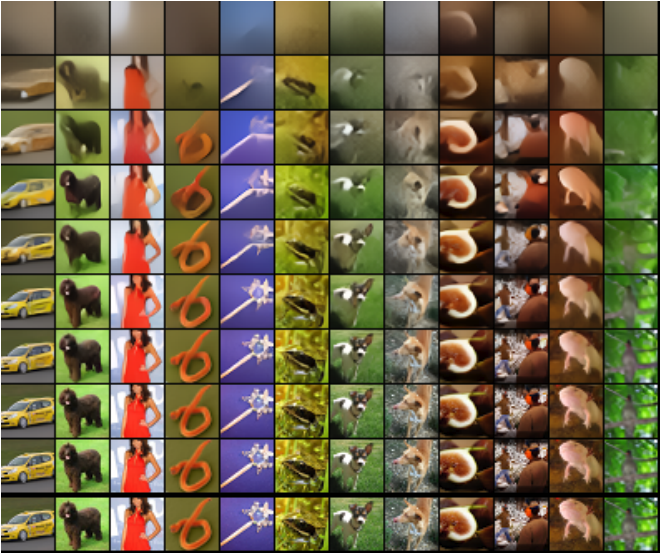
\includegraphics[width=0.66\textwidth]{figures/applications/conceptual_compression_gregor.png}
    \caption{Konceptuální komprese s použitím VAE aplikovaná na přirozené obrázky z ImageNet datasetu. Poslední řádek představuje originální obrázky. Zbylé řádky představují \textbf{komprimované} (shora dolů se snižuje počet latentních proměnných) rekonstrukce DRAW modelu. Převzato z \textcite{Gregor2016}.}
    \label{fig:conceptual_compression_gregor}
\end{figure}

Jelikož značný počet bitů každého obrázku slouží jako nositel těchto \emph{detailnějších} atributů, lze jejich zanedbání využít za účelem ztrátové komprese pomocí VAE.

Model konceptuální komprese založený na rozšíření VAE nabízí \textbf{větší kvalitu než kompresní algoritmy JPEG a JPEG 2000}
\footnote{Aktuálně je stále nejspolehlivějším arbitrem pro posouzení kvality ztrátové komprese člověk. Jiné (dostatečně jednoduché) míry, jako například L2 vzdálenost, jsou nevhodné. \cite{Gregor2016}} ve všech úrovních detekovatelné korupce výsledného obrázku (pro detailnější srovnání viz \textcite{Gregor2016}).

\newpage
\section{Syntéza přirozeného jazyka}
\label{sec:applications_language_synthesis}
Aplikací VAE na \textbf{interpolaci mezi větami přirozeného jazyka} představuje \textcite{Bowman2016}.

Zde je jednoduchý VAE (se stejnou strukturou, jakou prezentuje \autoref{chap:vae}) trénován na korpusu přirozeného anglického jazyka.

\begin{figure}[H]
    \centering
    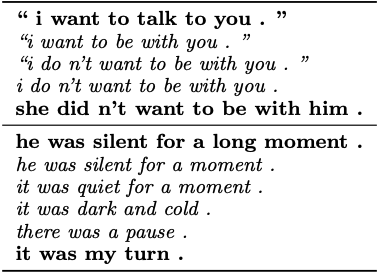
\includegraphics[width=0.9\textwidth]{figures/applications/vae_sentence_interpolation_bowman.png}
    \caption{Aplikace VAE pro interpolaci přirozeného jazyka mezi dvojicí vět. Vstupní páry vět jsou vyznačeny tučně, přechodné věty vygenerované modelem VAE jsou kurzívou.
    Pozoruhodně jsou přechodné věty \textbf{gramaticky i syntakticky správné} a \textbf{zachovávají tématický kontext} vstupních párů vět. Převzato z \textcite{Bowman2016}.}
    \label{fig:vae_sentence_interpolation_bowman}
\end{figure}

Výsledkem je model, který je schopen úspěšně \textbf{interpolovat mezi větami} a \textbf{doplnit do vět chybějící slova}. \autoref{fig:vae_sentence_interpolation_bowman} prezentuje schopnost takto naučeného modelu k interpolaci mezi vstupními páry vět. \cite{Bowman2016}

\newpage
\section{Návrh chemikálií}
\label{sec:applications_chemical_pseudo_data_synthesis}
Doposud byly prezentovány spíše ilustrační využití VAE. Nicméně rámec VAE nalézá uplatnění i pro vědecké účely.
 

\textcite{GomezBombarelli2018} představují jednoduchý VAE, který je trénován na datové sadě obsahující stovky tisíc existujících chemických struktur.
Tento VAE má stejnou strukturou modulů, jako popisuje \autoref{chap:vae}.
Výsledný latentní prostor (a jeho spojitá reprezentace) je posléze použit k gradientní optimalizaci cílového modelu směrem k určitým (chtěným) vlastnostem (viz \textcite{GomezBombarelli2018}).

\begin{figure}[H]
    \centering
    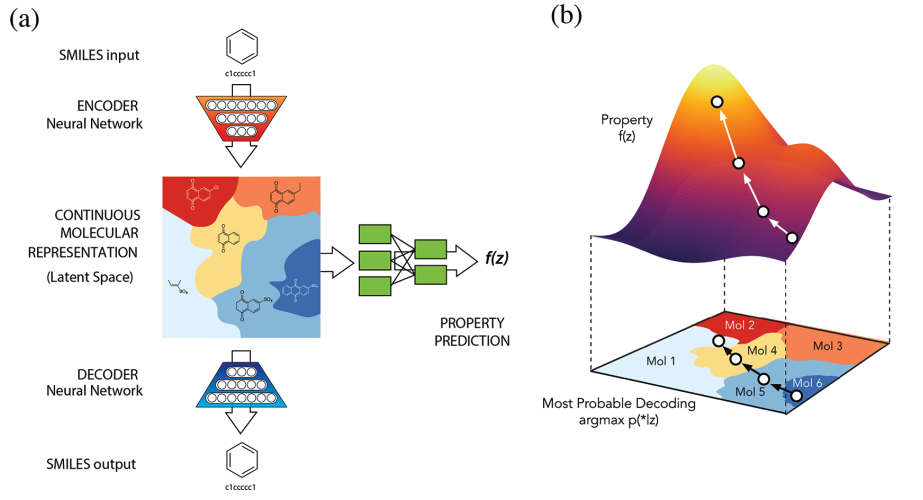
\includegraphics[width=\textwidth]{figures/applications/vae_molecule_design_gomez.png}
    \caption{Aplikace VAE k návrhu chemikálií. Obrázek (a): Proces naučení latentní spojité reprezentace molekul $\mathbf{z}$ z velkého vstupního datasetu. Obrázek (b): Takto naučená spojitá reprezentace umožňuje hledání nových molekul které maximalizují $f(z)$ (určitou \emph{vyžadovanou} vlastnost molekul). Převzato z \textcite{GomezBombarelli2018}.}
    \label{fig:vae_molecule_design_gomez}
\end{figure}

Princip této metody k návrhu molekul léků (či alespoň přidružených molekul) demonstruje \autoref{fig:vae_molecule_design_gomez}. \cite{Kingma2019}

\newpage
\section{Astronomie}
\label{sec:applications_astronomy_pseudo_data_synthesis}
Další aplikací VAE v oblasti vědy prezentuje \textcite{Ravanbakhsh2016}.
Autoři aplikují VAE k simulaci pozorování vzdálených galaxií.
Vzorky generované VAE pomáhají kalibrovat systémy, jejichž úkolem je detekovat zkreslení pozorování těchto galaxií (tzv. \emph{shearing}). Toto zkreslení je způsobeno jevem gravitační čočky
\footnote{Pojem gravitační čočky vychází ze spojné (optické) čočky. Užívá se pro popis objektu (např. klastru galaxií), který vlivem svého gravitačního pole způsobuje prohnutí paprsků světla vycházejících ze zdroje směrem k pozorovateli.},
který vzniká vlivem přítomnosti temné hmoty mezi Zemí a (pozorovanými) galaxiemi. \cite{Kingma2019}

\begin{figure}[H]
    \centering
    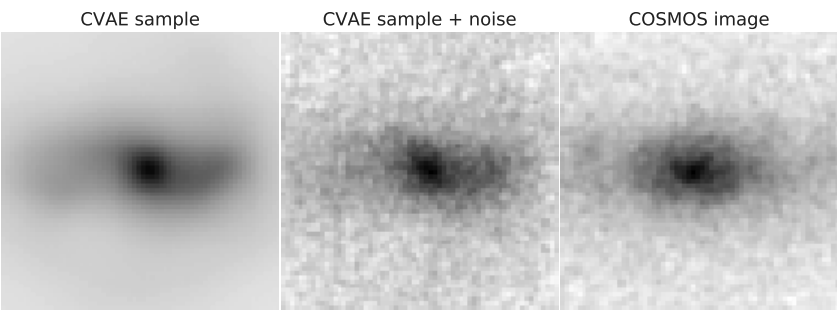
\includegraphics[width=0.9\textwidth]{figures/applications/vae_space_pseudodata_ravanbakhsh.png}
    \caption{Aplikace VAE k generování syntetických pseudo dat využitelných pro kalibraci systému k detekci zkreslení pozorování galaxií. K vygenerovanému vzorku pozorování je dodatečně přidán šum. Obrázek vlevo představuje vzorek z generativního modelu, obrázek vpravo představuje reálný snímek pozorování. Převzato z \textcite{Ravanbakhsh2016}.}
    \label{fig:vae_space_pseudodata_ravanbakhsh}
\end{figure}


Vzhledem k tomu, že jev gravitační čočky je opravdu slabý (a tím pádem složitě detekovatelný), je nutné tyto systémy kalibrovat \textbf{realistickými} obrázky s odpovídajícím množství zkreslení.
A vzhledem k tomu, že dostupné \textbf{množství} takových \textbf{reálných dat je aktuálně velmi omezené}, přistoupili autoři studie k využití VAE (respektive CVAE, viz \autoref{sec:cvae}) za účelem \textbf{syntézy pseudo-dat}, které jsou následně pro kalibraci využity. Jeden takový vzorek prezentuje \autoref{fig:vae_space_pseudodata_ravanbakhsh}. \cite{Ravanbakhsh2016}
